\documentclass[11.5pt]{beamer}
\usepackage[numbers,sort&compress]{natbib}
\usepackage{amsmath,amssymb,amsfonts,amsthm}
\usepackage{algorithm,setspace}
\usepackage{algpseudocode}
\usepackage{caption}
\usepackage{hyperref} 

\renewcommand{\algorithmicrequire}{\textbf{Input:}} 
\renewcommand{\algorithmicensure}{\textbf{Output:}} 

\setbeamertemplate{theorems}[numbered]
\setbeamerfont{frametitle}{series=\bfseries,parent=structure}
\newtheorem{assumption}{Assumption}


\usetheme{Boadilla}
\author[X. Li, C. Wu, \& Y. Huang]{Xiaopeng Li, Chenhao Wu \& Yihan Huang}
\title{Trajectory and Power Control for UAVs}
\institute[CUHK(SZ)]{The Chinese University of Hong Kong, Shenzhen}
\date{\today}

\begin{document}

\frame{\titlepage}

\begin{frame}
	\frametitle{Outline}
	\tableofcontents
\end{frame}

\section{Introduction}
\begin{frame}
	\frametitle{Introduction}
	\begin{figure}
		\centering
		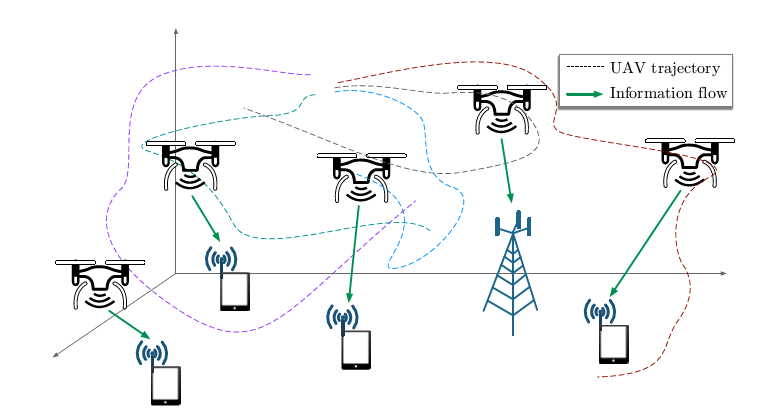
\includegraphics[width=.9\linewidth]{Intro_figure.png}
	\end{figure}
\end{frame}


\begin{frame}
	\frametitle{Introduction}
	\begin{itemize}\itemsep4em
		\item<1-> Practical constraints
		\begin{itemize}
			\item Transmission interference
			\item Limited speed and altitude
			\item Collision
		\end{itemize}
		\item<2-> TPC Problem
		\begin{itemize}
			\item Joint trajectory optimizaiton
			\item Power control
		\end{itemize}
	\end{itemize}
\end{frame}


\section{Problem Formulation}
\begin{frame}
	\frametitle{Problem Formulation}
	\begin{itemize}\itemsep4em
		\item<1-> BS position
		\begin{itemize}
			\item Fixed base station (BS) position: $\boldsymbol{s}\in\mathbb{R}^{3\times K}$
			\item $k$-th BS position: $\boldsymbol{s}[:,k]\in\mathbb{R}^3,\,\forall\,k\in\mathcal{K}$
				, where $\mathcal{K}\triangleq\{1,\ldots,K\}$
		\end{itemize}
		\item<2-> UAV location
		\begin{itemize}
			\item UAV location: $\boldsymbol{q}\in\mathbb{R}^{3\times K\times (N+2)}$
			\item $k$-th UAV at time slot $n$: $\boldsymbol{q}[:,k,n+1]\in\mathbb{R}^3$ for $n\in\mathcal{N}_1^N$
				, where $\mathcal{N}_i^j=\{i,\ldots,j\}$
			\item Initial location: $\boldsymbol{q}[:,k,1]$
			\item Final location: $\boldsymbol{q}[:,k,N+2]$
		\end{itemize}
	\end{itemize}
\end{frame}


\begin{frame}
	\frametitle{Problem Formulation}
	\begin{itemize}\itemsep2em
		\item<1-> Altitude constraint
		\begin{itemize}
			\item Minimum and maximum safe altitude for all UAV: $H_{\min}$ and $H_{\max}$
			\item Altitude constraint: 
				\begin{equation}\label{Eq1}
					H_{\min}\leq\boldsymbol{q}[3,k,n+1]\leq H_{\max}
				\end{equation}
		\end{itemize}
		\item<2-> Speed constraint
		\begin{itemize}
			\item Level-flight speed, vertical ascending and descending speed: $V_L,V_A$ and $V_D$
			\item Position constraints:
				\begin{subequations}
					\begin{equation}\label{Eq2.1}
						\left\lVert\boldsymbol{q}[1:2,k,n+1]-\boldsymbol{q}[1:2,k,n]\right\rVert\leq V_LT_s
					\end{equation}
					\begin{equation}\label{Eq2.2}
						-V_DT_s\leq\boldsymbol{q}[3,k,n+1]-\boldsymbol{q}[3,k,n]\leq V_AT_s
					\end{equation}
				\end{subequations}
		\end{itemize}
	\end{itemize}
\end{frame}


\begin{frame}
	\frametitle{Problem Formulation}
	\begin{itemize}\itemsep2em
		\item<1-> Collision avoidance
		\begin{itemize}
			\item Minimum safety distance between any two UAVs: $d_{\min}$
			\item Collision avoidance constraints:
				\begin{equation}\label{Eq3}
					\left\lVert\boldsymbol{q}[:,k,n+1]-\boldsymbol{q}[:,j,n+1]\right\rVert\geq d_{\min}
				\end{equation}
		\end{itemize}
		\item<2-> Power constraint
		\begin{itemize}
			\item Transimission power of UAV: $\boldsymbol{p}\in\mathbb{R}^{k\times (N+2)}$
			\item $k$-th UAV at time slot $n$: $\boldsymbol{p}[k,n+1]\in\mathbb{R}$
			\item Maximum transimission power: $P_{\max}$
			\item Power constraint:
				\begin{equation}\label{Eq4}
					0\leq \boldsymbol{p}[k,n+1]\leq P_{\max}
				\end{equation}
		\end{itemize}
	\end{itemize}
\end{frame}


\begin{frame}
	\frametitle{Problem Formulation}
	\begin{itemize}\itemsep4em
		\item<1-> Objective function 
		\begin{itemize}
			\item Channel capacity (bits/second): $R\in\mathbb{R}^{K\times (N+2)}$
			\item $k$-th UAV at time slot $n$: $R_{[k,n+1]}\in\mathbb{R}$, for $k\in\mathcal{K}$ and $n\in\mathcal{N}_1^N$
			\item TPC optimization problem: 
				\begin{equation} 
					\begin{array}{cll}
						\max\limits_{\substack{\boldsymbol{p}_{[:,2:N+1]},\\ \boldsymbol{q}_{[:,:,2:N+1]}}}\quad & 						\sum\limits_{n=2}^{N+1}\sum\limits_{k=1}^K R_{[k,n]}(\boldsymbol{p},\boldsymbol{q}) \\ 
						s.t. \quad & (\ref{Eq1}),(\ref{Eq4})\ \forall\,k\in\mathcal{K},n\in\mathcal{N}_1^N \\
						& (\ref{Eq2.1}),(\ref{Eq2.2}),\ \forall\,k\in\mathcal{K},n\in\mathcal{N}_1^{N+1} \\
						& (\ref{Eq3}),\ \forall\,k,j\in\mathcal{K},k<j,n\in\mathcal{N}_1^N
					\end{array}
				\end{equation}
		\end{itemize}
	\end{itemize}
\end{frame}


\begin{frame}
	\frametitle{Problem Formulation}
	\begin{itemize}\itemsep2em
		\item<1-> $R_{[k,n]}$: Channel capacity
		\begin{itemize}
			\item Bandwidth of channel (Hz): $B$
			\item Signal-to-noise ratio: SNR
			\item Channel capacity:
				\begin{equation}
					R_{[k,n]} = B\log_2\left(1+\text{SNR}_{[k,n]}\right)\tag{5.1}
				\end{equation}
		\end{itemize}
		\item<2-> SNR: Signal-to-noise ratio
		\begin{itemize}
			\item Channel gain: $G\in\mathbb{R}^{K\times K\times (N+2)}$
			\item Power spectral density of AWGN: $N_0$
			\item SNR:
				 \begin{equation}\label{Eq5.2}
					\text{SNR}_{[k,n]} = \frac{G_{[k,k,n]}\boldsymbol{p}_{[k,n]}}{BN_0+\sum_{j=1,j\ne k}^{K}    G_{[j,k,n]}\boldsymbol{p}_{[j,n]}}\tag{5.2}
				 \end{equation}
		\end{itemize}
	\end{itemize}
\end{frame}


\begin{frame}
	\frametitle{Problem Formulation}
	\begin{itemize}\itemsep4em
		\item<1-> $G_{[k,k,n]}$: Power gain
		\begin{itemize}
			\item Channel gain beween UAV and BS: $G\in\mathbb{R}^{K\times K\times (N+2)}$
			\item Channel gain between any UAV and BS at one meter: $G_0$
			\item Channel gain between $j$-th UAV and $k$-th BS at time slot $n$:
				\begin{equation}\label{Eq5.3}
					G_{[j,k,n+1]}=\frac{G_0}{\lVert\boldsymbol{q}_{[:,j,n+1]}-\boldsymbol{s}_{[:,k]}\rVert^2} 	 						\tag{5.3}
				\end{equation}
		\end{itemize}
	\end{itemize}
\end{frame}


\begin{frame}
	\frametitle{Problem Formulation}
	\begin{itemize}\itemsep4em
		\item<1-> Notice
		\begin{itemize}
			\item UAV should return to its initial position: 
				\begin{equation}\label{6.1}
					\boldsymbol{q}_{[:,k,1]} = \boldsymbol{q}_{[:,k,N+2]},\ \forall\,k\in\mathcal{K}\tag{6.1}
				\end{equation}
			\item Time slot short enough to avoid collision:
				\begin{equation}\label{6.2}
					T_s \leq \frac{d_{\min}}{\sqrt{4V_L^2+(V_A+V_D)^2}}\tag{6.2}
				\end{equation}
		\end{itemize}
	\end{itemize}
\end{frame}

\section{Main Strategies}
\begin{frame}
	\frametitle{Main Strategies}
	\begin{itemize}\itemsep4em
		\item<1-> Two main difficulties
		\begin{itemize}
			\item Large problem dimension
			\item Non-convex optimization
		\end{itemize}
		\item<2-> Two main strategies
		\begin{itemize}
			\item Heuristic dimension-reduced method
			\item Successive convex approximation (SCA)
		\end{itemize}
	\end{itemize}
\end{frame}


\begin{frame}
\frametitle{Main Strategies}
	\begin{block}<1->{Fly-hover-fly Strategy}
		The fly-hover-fly strategy is described as
		\begin{itemize}
			\item UAVs fly to the hovering location.
			\item UAVs hover over that location.
			\item UAVs return to the original position from the hovering location.
		\end{itemize}
	\end{block}
	\vskip 2\baselineskip
	\begin{assumption}<2->
		The whole time horizon $T$ is \alert{much longer} than the time UAVs need to fly to the hovering location.
	\end{assumption}
\end{frame}


\begin{frame}
\frametitle{Main Strategies}
	\begin{lemma}\label{lemma1}
		Assume all UAVs return to the initial locations, and the ascending and descending speed are equal, i.e., $V_A=V_D$. Denote one of the optimal solution of TPC problem as $\boldsymbol{q}^*$ and $\boldsymbol{p}^*$, then for all $k\in\mathcal{K},n\in\mathcal{N}_2^{N+2}$,
		\begin{equation}\label{lemma1eq}
			\boldsymbol{q}^*_{[:,k,n]} = \boldsymbol{q}^*_{[:,k,N+3-n]},\ \boldsymbol{p}^*_{[k,n]} = \boldsymbol{p}^*_{[k,N+3-n]}
		\end{equation}
	\end{lemma}
\end{frame}


\begin{frame}
\frametitle{Main Strategies}
	\begin{lemma}
		Using the same notations in {\rm Lemma \ref{lemma1}}, for some $M_0\in\{2,3,\ldots,N+1\}$ and $M\in\{2,3,\ldots,M_0\}$, we have
		\begin{equation}\label{lemma2eq}
			{R_s}_{[n]}\leq {R_s}_{[M]}={R_s}_{[M+1]}=\cdots={R_s}_{[M_0]},\ \forall\,n\in\mathcal{N}_2^M
		\end{equation}
		where $M_0$ is the time when the UAVs need to return from the hovering location, and $M$ is the time when UAVs arrives the hovering location. In particular, if $V_A=V_D$, $M_0=N+3-M$.
	\end{lemma}
\end{frame}


\begin{frame}
\frametitle{Main Strategies}
	\begin{itemize}
		\item<1-> Reformulation 1
		\begin{equation}\label{reformulation1}
			\begin{array}{cll}
			\max\limits_{\substack{\boldsymbol{p}_{[:,2:M]}, \\ \boldsymbol{q}_{[:,:,2:M]}, \\ M\in\mathcal{N}_2^{(N+1)/2}}}\quad & \sum\limits_{n=2}^{M}\sum\limits_{k=1}^K R_{[k,n]}(\boldsymbol{p},\boldsymbol{q}) \\[-20pt] &\qquad+\left(\frac{N+1}{2}-M\right)\sum\limits_{k=1}^KR_{[k,M]}(\boldsymbol{p},\boldsymbol{q}) \\
			s.t. \quad & (\ref{Eq1}),(\ref{Eq2.1}),(\ref{Eq2.2}),(\ref{Eq4}),\ \forall\,k\in\mathcal{K},n\in\mathcal{N}_2^M \\
			& (\ref{Eq3}),\ \forall\,k,j\in\mathcal{K},k<j,n\in\mathcal{N}_2^M
			\end{array}
		\end{equation}
		\item<2-> Reformulation 2
		\begin{equation}\label{reformulation2}
			\begin{array}{cl}
			\max\limits_{\substack{\boldsymbol{p}_{[:,2:M]}, \\ \boldsymbol{q}_{[:,:,2:M]} \\ M\in\mathcal{N}_2^{(N+1)/2}
			}} & \sum\limits_{n=2}^{M}\sum\limits_{k=1}^K R_{[k,n]}(\boldsymbol{p},\boldsymbol{q}) \\[-13pt] &\qquad+(\frac{N+1}{2}-M)R_s^* \\[5pt]
			s.t.  & (\ref{Eq1}),(\ref{Eq2.1}),(\ref{Eq2.2}),(\ref{Eq4}),\ \forall\,k\in\mathcal{K},n\in\mathcal{N}_2^M \\
			& (\ref{Eq3}),\ \forall\,k,j\in\mathcal{K},k<j,n\in\mathcal{N}_2^M \\
			& \boldsymbol{q}_{[:,k,M]}=\boldsymbol{q_h}^*_{[:,k]},\   \boldsymbol{p}_{[k,M]} = \boldsymbol{p_h}^*_{[k]},\  \forall\,k\in\mathcal{K}
			\end{array}
		\end{equation}
	\end{itemize}
\end{frame}


\begin{frame}
\frametitle{Main Strategies}
	\begin{itemize}
		\item<1-> \alert{Successive convex approximation.} Find a locally tight convex surrogate function to replace the objective function or constraints.
		\item<2-> Trick. \alert{First-order Taylor's expansion.}
		\begin{subequations}
			\begin{flalign*}
			&\frac{x^2}{y} \geq \frac{2\bar{x}}{\bar{y}}x-\frac{\bar{x}^2}{\bar{y}^2}y,\ \text{for fixed }\bar{y}>0 \\
			&-\log(1+x) \geq -\log(1+\bar{x}) - \frac{x-\bar{x}}{1+\bar{x}} \\
			&x^2 \geq 2x\bar{x}-\bar{x}^2
			\end{flalign*}
		\end{subequations}
		\item<3-> Objective function. 
		\begin{equation}\label{obj2}
			\begin{array}{rl}
				\overline{R}[k,n](\boldsymbol{a},\boldsymbol{q}) \triangleq & \log\left(1+\sum_{j=1}^K\frac{G_0(\boldsymbol{a}[k,j])^2}{BN_0\boldsymbol{d}[j,k,n]}\right)\\
				&\qquad-\log\left(1+\sum_{j=1,j\ne k}^K\frac{G_0(\boldsymbol{a}[k,j])^2}{BN_0\boldsymbol{d}[j,k,n]}\right)
			\end{array}
		\end{equation}
	\end{itemize}
\end{frame}

\begin{frame}
	\frametitle{Main Strategies}
	\begin{itemize}
		\item<1-> Surrogate function. 
		\begin{equation}\label{surro}
			\begin{array}{ll}
			\widetilde{R}_{[k,n]}(\boldsymbol{a},\boldsymbol{q};\boldsymbol{a}^r,\boldsymbol{q}^r) \triangleq\log\left(1+\frac{G_0}{BN_0}\sum\limits_{j=1}^K\left[\frac{2\boldsymbol{a}^r_{[j,n]}}{\boldsymbol{d}^r_{[j,k,n]}}\boldsymbol{a}_{[j,n]}\right.\right. \\
			\left.\left.-\frac{(\boldsymbol{a}^r_{[k,j]})^2}{(\boldsymbol{d}^r_{[j,k,n]})^2}\lVert\boldsymbol{q}_{[:,j,n]}-\boldsymbol{s}_{[:,k]}\rVert^2\right]\right)-\log(1+\boldsymbol{I}^r_{[k,n]})+\frac{\boldsymbol{I}^r_{[k,n]}}{1+\boldsymbol{I}^r_{[k,n]}} \\
			-\frac{G_0}{BN_0(1+\boldsymbol{I}^r_{[k,n]})}\sum\limits_{j=1,j\ne k}^{K}\frac{(\boldsymbol{a}_{[j,n]})^2}{\boldsymbol{d}^r_{[j,k,n]}+2(\boldsymbol{q}^r_{[:,j,n]}-\boldsymbol{s}_{[:,k]})^{\rm T}(\boldsymbol{q}_{[:,j,n]}-\boldsymbol{q}^r_{[:,j,n]})}
			\end{array}
		\end{equation}
		\item<2-> Collision avoidance constraint
		\begin{equation}\label{cstr}
			\begin{array}{c}
			2(\boldsymbol{q}^r_{[:,k,n]}-\boldsymbol{q}^r_{[:,j,n]})^{\rm T}(\boldsymbol{q}_{[:,k,n]}-\boldsymbol{q}_{[:,j,n]})\geq  \\
			\qquad\qquad\qquad\qquad\qquad\left\lVert\boldsymbol{q}^r_{[:,k,n]}-\boldsymbol{q}^r_{[:,j,n]}\right\rVert^2+d_{\min}^2
			\end{array}
		\end{equation}
	\end{itemize}
\end{frame}


\begin{frame}
\frametitle{Main Strategies}
Therefore, the convex approximation problem for (\ref{reformulation2}) given $M$ is
\begin{equation}\label{cvxapprox}
	\begin{array}{cll}
	\max\limits_{\substack{\boldsymbol{a}_{[:,2:M]},\\ \boldsymbol{q}_{[:,:,2:M]}}}\quad & \sum\limits_{n=2}^{M}\sum\limits_{k=1}^K \widetilde{R}_{[k,n]}(\boldsymbol{a},\boldsymbol{q};\boldsymbol{a}^r,\boldsymbol{q}^r) \\ 
	s.t.  & (\ref{Eq1}),(\ref{Eq2.1}),(\ref{Eq2.2}),(\ref{Eq4}),\ \forall\,k\in\mathcal{K},n\in\mathcal{N}_2^M \\
	& (\ref{cstr}),\ \forall\,k,j\in\mathcal{K},k<j,n\in\mathcal{N}_2^M \\
	& \boldsymbol{q}_{[:,k,M]}=\boldsymbol{q_h}^*_{[:,k]},\   \boldsymbol{p}_{[k,M]} = \boldsymbol{p_h}^*_{[k]},\  \forall\,k\in\mathcal{K}
	\end{array}
\end{equation}

\end{frame}


\begin{frame}
\frametitle{Main Strategies}

\begin{algorithm}[H]
	\caption{SCA algorithm for solving problem (\ref{reformulation2})}
	\label{alg:1}
	\scriptsize
	\setstretch{1.5}
	\begin{algorithmic}[1]
		\State {Set iteration index $r=0$, tolerance $\epsilon>0$.} 
		\State {Initialize $\boldsymbol{q}^0_{[:,k,n]}$ and $\boldsymbol{p}^0_{[k,n]}$ for $k\in\mathcal{K},n\in\mathcal{N}_2^M$.}
		\State {Calculate $R^0=\sum_{k=1}^K\sum_{n=2}^MR_{[k,n]}(\boldsymbol{p}^0,\boldsymbol{q}^0)$.}
		\Repeat 
		\State Calculate $\left\{\boldsymbol{a}^r_{[k,n]},\boldsymbol{d}^r_{[j,k,n]},\boldsymbol{I}^r_{[k,n]}\right\}$ by using $\boldsymbol{p}^r_{[k,n]}$ and $\boldsymbol{q}^r_{[:,k,n]}$.
		\State Update $\left\{\boldsymbol{a}^{r+1}_{[k,n]},\boldsymbol{q}^{r+1}_{[:,k,n]}\right\}$ by solving problem (\ref{cvxapprox}) with parameters $\boldsymbol{a}^r_{[k,n]}$, $\boldsymbol{d}^r_{[j,k,n]}$, and $\boldsymbol{I}^r_{[k,n]}$.
		\State Calculate $\boldsymbol{p}^{r+1}_{[k,n]}$ by using $\boldsymbol{a}^{r+1}_{[k,n]}$.
		\State Set $r=r+1$.
		\Until{$\frac{|R^r-R^{r-1}|}{R^{r-1}}\leq\epsilon$} \\
		\Return{$\left\{\boldsymbol{p}^r_{[k,n]},\boldsymbol{q}^r_{[:,k,n]}\right\}$}
	\end{algorithmic}
\end{algorithm}

\end{frame}

\section{Simulation Result}
\begin{frame}
	\frametitle{Simulation Result}
	
	\begin{itemize}
		\item<1-> Simulation Scale
		\begin{itemize}
			\item \# of UAV-BS pairs: $K = 4$
			\item \# of time slots: $M = 160$
		\end{itemize}
		\item<2-> Parameter Setup
		\begin{itemize}
			\item $d_{\text{min}} = 20 m$
			\item $V_L = 20 m/s$, $V_A = V_D = 5 m/s$ 
			\item $h_{\text{min}} = 100m$, $h_{\text{max}} = 200m$
			\item $P_{\text{max}} = 30dbm$
			\item Communication bandwidth: $B = 10 MHz$
			\item Power spectral density of addictive white Gaussian noise: $N_0 = -160 dbm/Hz$
		\end{itemize}
		\item<3-> Initial locations
		\begin{itemize}
			\item UAV: (0, 0, 100), (30, 0, 100), (0, 30, 100), (30, 30, 100)
			\item Base station: (300, 0, 0), (100, 600, 0), (700, 700, 0), (100, 800, 0)
		\end{itemize}
	\end{itemize}
	\quad \quad \scriptsize Source Code: \href{https://github.com/Vito-Swift/EIE3280-CourseProj-TPC}{\underline{\textit{https://github.com/Vito-Swift/EIE3280-CourseProj-TPC}}}\\
\end{frame}
\begin{frame}
	\frametitle{Simulation Result}
	\begin{itemize}
		\item Initial trajectory
		\begin{itemize}
			\item Step 1: obtain the hovering points $q_{[:, k, M]}^*$ and the transmission powers $p_{[k, M]}^*$
			\item Step 2: obtain $M^*$ and the initial trajectory $q_{[:, k, n]}^0$
		\end{itemize}
	\end{itemize}
	
	\begin{figure}
		\centering
		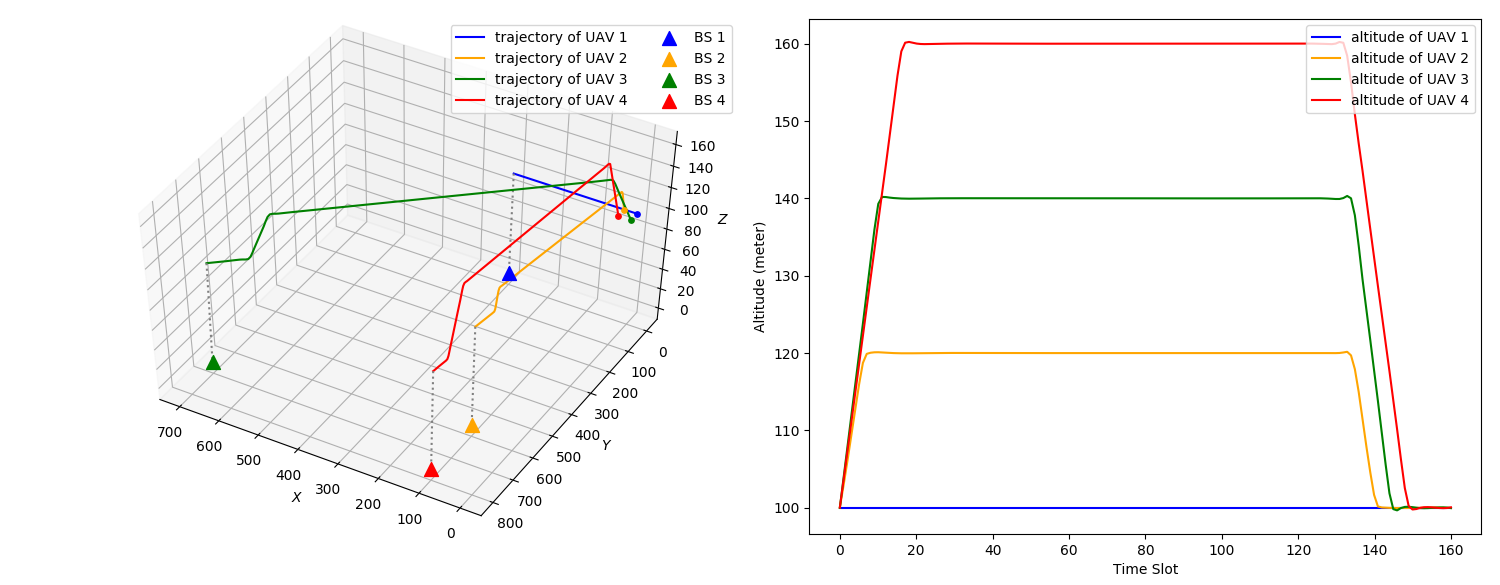
\includegraphics[width=.9\linewidth]{init_trajectory.png}
	\end{figure}
\end{frame}
\begin{frame}
	\frametitle{Simulation Result}
	\begin{itemize}\itemsep-0.5em
		\item Initial trajectory
		\begin{figure}
			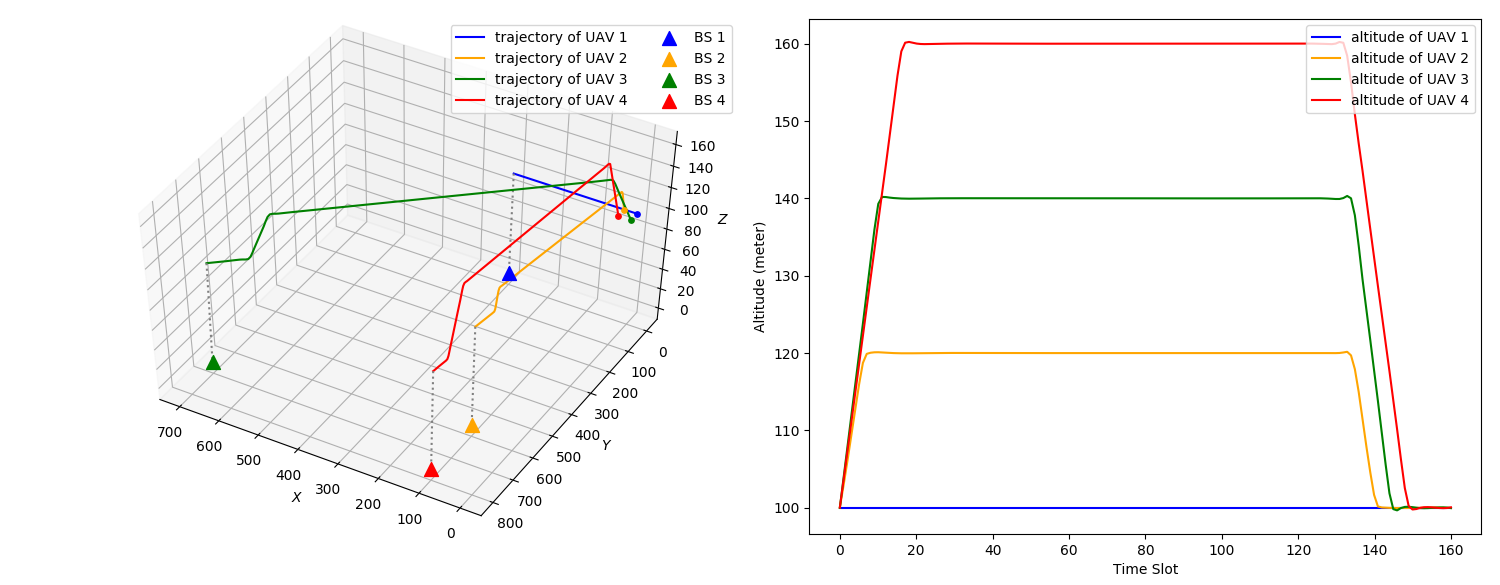
\includegraphics[width=.8\linewidth]{init_trajectory.png}
		\end{figure}
		\item Optimized trajectory
		\begin{figure}
			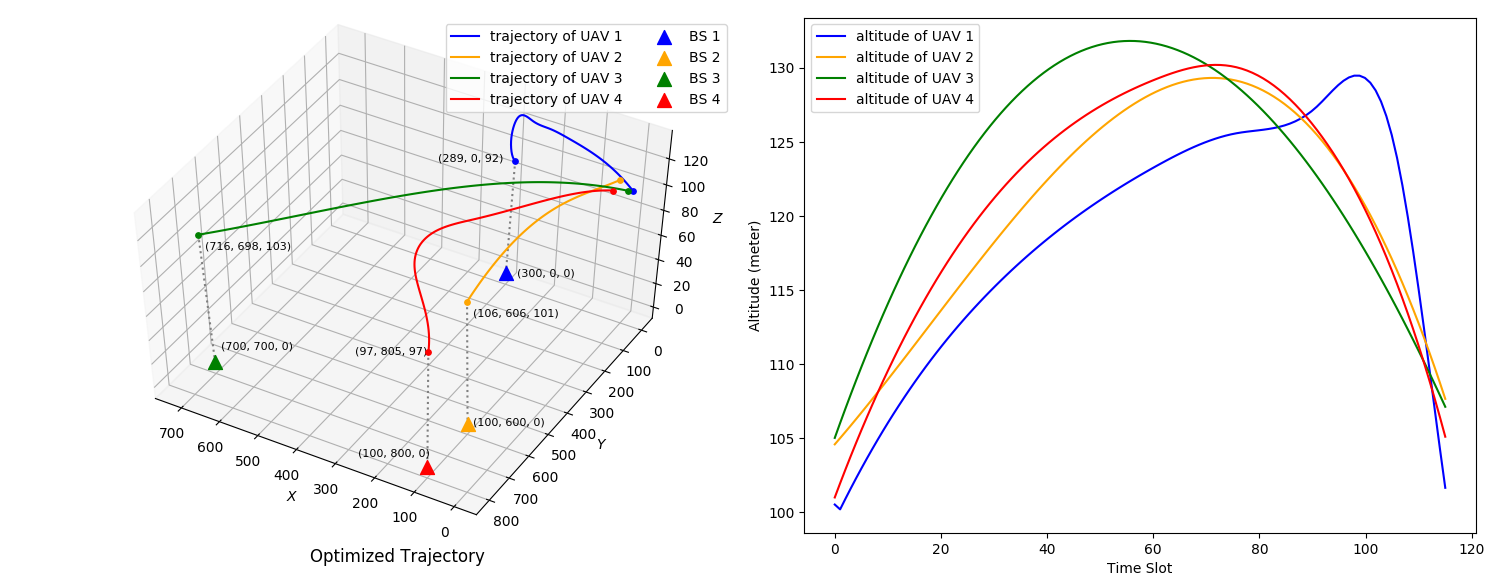
\includegraphics[width=.8\linewidth]{opt_trajectory.png}
		\end{figure}
	\end{itemize}
\end{frame}
\begin{frame}
	\frametitle{Simulation Result}
	\begin{itemize}\itemsep-0.5em
		\item Initial achievable transmission rate
		\begin{figure}
			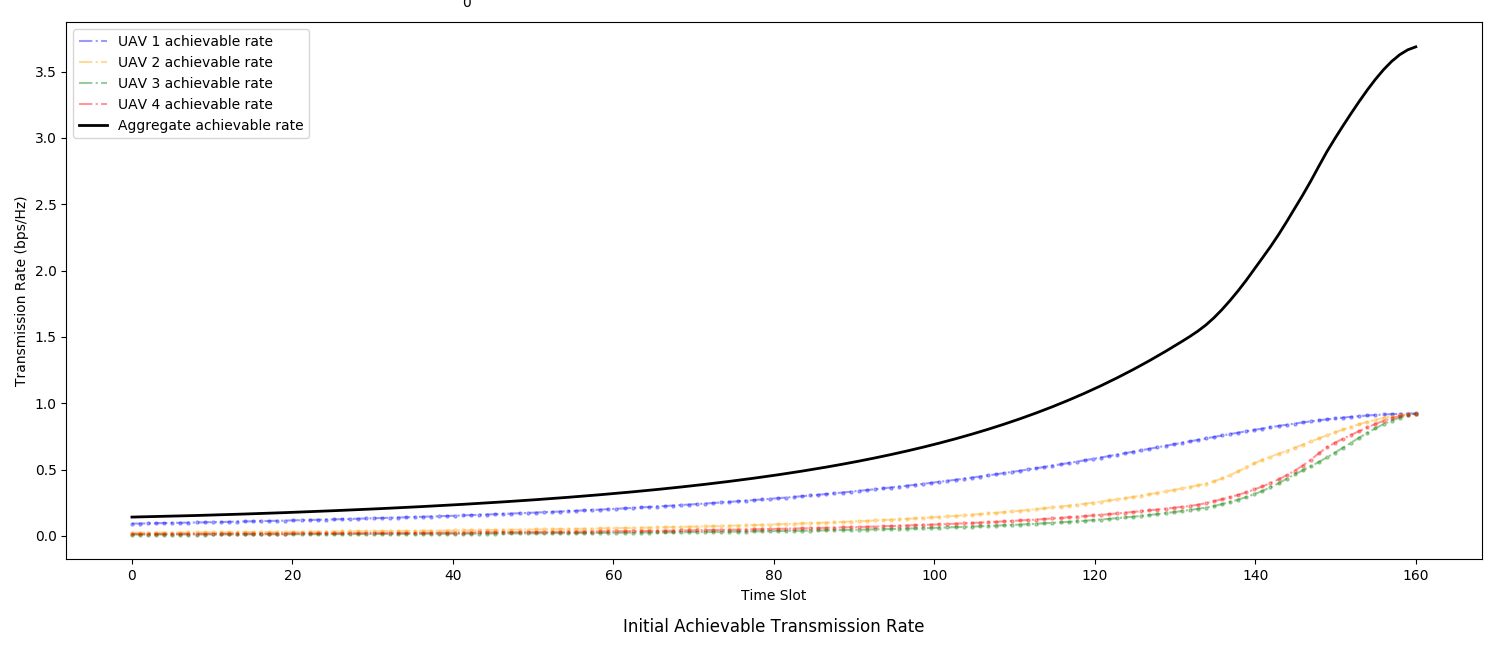
\includegraphics[width=.7\linewidth]{init_rate.png}
		\end{figure}
		\item Optimized achievable transmission rate
		\begin{figure}
			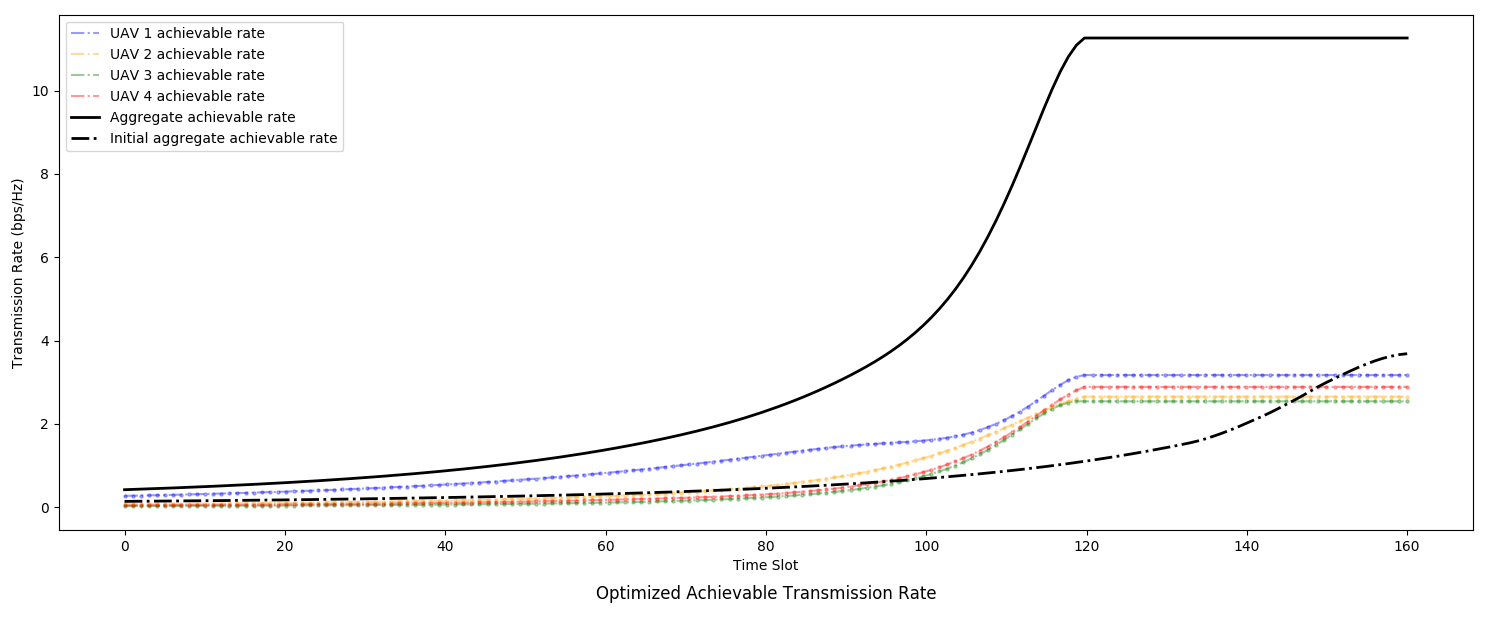
\includegraphics[width=.7\linewidth]{opt_rate.png}
		\end{figure}
	\end{itemize}
\end{frame}

\section{Conclusion}
\begin{frame}
	\frametitle{Conclusion}
	\begin{itemize}\itemsep 2em
		\item<1-> Generally, TPC problem is NP-hard and we apply an efficient SCA-based suboptimal algorithms to optimize the initial trajectory and power control.
		\item<2-> From simulations,
		\begin{itemize}
			\item the aggregate transmission rate raised
			\item UAV approaches $q^*$ in a more preferable route 
			\begin{itemize}
				\item shorter traveling duration
				\item lower maximum height
			\end{itemize}
		\end{itemize}
	\end{itemize}
\end{frame}
\begin{frame}
	\frametitle{Conclusion}
	\begin{itemize}
		\item Future Work
		\begin{itemize}\itemsep 0.5em
			\item Perform simulations in more sophisticated scenarios
			\item Apply ADMM algorithm to modify our original algorithm, in order to reduce the computation overhead by using parallel computing
			\item From one antenna to multiple antennas - extend the current work to scenarios with multi-antenna base stations and UAVs 
		\end{itemize}
	\end{itemize}
\end{frame}

\begin{frame}{References}
	\nocite{IEEEexample:shen2018multi}
	\nocite{IEEEexample:zeng2016wireless}
	\nocite{IEEEexample:7888557}
	\nocite{IEEEexample:li2019uav}
	\bibliographystyle{IEEEtran}
	\bibliography{IEEEabrv,IEEEexample}
\end{frame}

	
	
	
	
	
	
	
\end{document}